\documentclass{beamer}
\usepackage{listings}
% \usepackage{pgfpages}
% \pgfpagesuselayout{4 on 1}[a4paper,border shrink=5mm,landscape]

\title{High-Performance Haskell}
\author{Johan Tibell\\johan.tibell@gmail.com}
\date{2010-10-01}

\begin{document}
\lstset{language=Haskell}

\frame{\titlepage}

\begin{frame}
  \frametitle{Welcome!}

  A few things about this tutorial:
  \begin{itemize}
  \item Stop me and ask questions---early and often
  \item I assume \emph{no} prior Haskell exposure
  \end{itemize}
\end{frame}

\begin{frame}
  \frametitle{Sequential performance is still important}

  Parallelism is not a magic bullet:
  \begin{itemize}
  \item The speedup of a program using multiple processors is limited
    by the time needed for the sequential fraction of the
    program. (Amdahl's law)
  \item We want to make \emph{efficient} use of every core.
  \end{itemize}
\end{frame}

\begin{frame}
  \frametitle{Caveats}

  The usual caveats about performance optimizations:
  \begin{itemize}
  \item Improvements to the compiler might make some optimizations
    redundant.  Write benchmarks to detect these cases.
  \item Some optimizations are compiler (i.e. GHC) specific
  \end{itemize}
  That being said, many of these optimizations have remained valid
  over a number of GHC releases.
\end{frame}

\begin{frame}[fragile]
  \frametitle{Software prerequisites}

  The Haskell Platform:
  \begin{itemize}
  \item Download installer for Windows, OS X, or Linux here:
  \item \url{http://hackage.haskell.org/platform}
  \end{itemize}

  The Criterion benchmarking library:
  \begin{verbatim}
cabal install -f-Chart criterion
  \end{verbatim}
\end{frame}

\begin{frame}
  \frametitle{Outline}

  \begin{itemize}
  \item Introduction to Haskell
  \item Lazy evaluation
  \item Reasoning about space usage
  \item Benchmarking
  \item Making sense of compiler output
  \item Profiling
  \end{itemize}
\end{frame}

\begin{frame}[fragile]
  \frametitle{Haskell in 10 minutes}

  Our first Haskell program sums a list of integers:
  \begin{lstlisting}
sum :: [Int] -> Int
sum []     = 0
sum (x:xs) = x + sum xs

main :: IO ()
main = print (sum [1..10000])
  \end{lstlisting}
\end{frame}

\begin{frame}[fragile]
  \frametitle{Type signatures}

  \begin{definition}
    A \alert{type signature} describes the type of a Haskell expression:
  \end{definition}

  \begin{lstlisting}
sum :: [Int] -> Int
  \end{lstlisting}
  \begin{itemize}
  \item \lstinline!Int! is an integer.
  \item \lstinline![a]! is a list of \lstinline!a!s
    \begin{itemize}
    \item So \lstinline![Int]! is a list of integers
    \end{itemize}
  \item \lstinline!->! denotes a function.
  \item So \lstinline!sum! is a function from a list of integers to an
    integer.
  \end{itemize}
\end{frame}

\begin{frame}[fragile]
  \frametitle{Defining a function}

  Functions are defined as a series of equations, using
  \emph{pattern matching}:

  \begin{lstlisting}
sum []     = 0
sum (x:xs) = x + sum xs
  \end{lstlisting}

  The list is defined recursively as either
  \begin{itemize}
  \item an empty list, written as \lstinline![]!, or
  \item an element \lstinline!x!, followed by a list \lstinline!xs!.
  \end{itemize}
  [] is pronounced ``nil'' and \lstinline!:! is pronounced ``cons''.
\end{frame}

\begin{frame}[fragile]
  \frametitle{Function application}

  Function application is indicated by \emph{juxtaposition}:

\begin{lstlisting}
main = print (sum [1..10000])
\end{lstlisting}

  \begin{itemize}
  \item \lstinline![1..10000]! creates a list of 10,000 integers from
    1 to 10,000.
  \item We apply the \lstinline!sum! function to the list and then
    apply the result to the print function.
  \end{itemize}

  We say that we \emph{apply} rather then \emph{call} a function:
  \begin{itemize}
  \item Haskell is a lazy language
  \item The result may not be computed immediately
  \end{itemize}
\end{frame}

\begin{frame}[fragile]
  \frametitle{Compiling and running our program}

  Save the program in a file called \lstinline!Sum.hs! and then
  compile it using \lstinline!ghc!:

\begin{verbatim}
$ ghc -O --make Sum.hs
[1 of 1] Compiling Main             ( Sum.hs, Sum.o )
Linking Sum ...
\end{verbatim}

Now lets run the program

\begin{verbatim}
$ ./Sum
50005000
\end{verbatim}
\end{frame}

\begin{frame}[fragile]
  \frametitle{Defining our own data types}

  Data types have one or more \emph{constructors}, each with zero or
  more \emph{arguments} (or \emph{fields}).

  \begin{lstlisting}
data Shape = Circle Double
           | Rectangle Double Double
  \end{lstlisting}

  And a function over our data type, again defined using pattern
  matching:
  \begin{lstlisting}
area :: Shape -> Double
area (Circle r)      = r * r * 3.14
area (Rectangle w h) = w * h
  \end{lstlisting}

  Constructing a value uses the same syntax as pattern matching:
\begin{lstlisting}
area (Rectangle 3.0 5.0)
\end{lstlisting}
\end{frame}

\begin{frame}[fragile]
  \frametitle{Back to our sum function}

  Our \lstinline!sum! has a problem. If we increase the size of the
  input

\begin{lstlisting}
main = print (sum [1..10000000])
\end{lstlisting}

and run the program again

\begin{verbatim}
$ ghc -O --make Sum.hs
[1 of 1] Compiling Main             ( Sum.hs, Sum.o )
Linking Sum ...
$ ./Sum
Stack space overflow: current size 8388608 bytes.
Use `+RTS -Ksize -RTS' to increase it.
\end{verbatim}
\end{frame}

\begin{frame}[fragile]
  \frametitle{Tail recursion}

  Our function creates a stack frame for each recursive call,
  eventually reaching the predefined stack limit.
  \begin{itemize}
  \item Must do so as we still need to apply + to the result of the
    call.
  \end{itemize}

  Make sure that the recursive application is the last thing in the
  function
  \begin{lstlisting}
sum :: [Int] -> Int
sum xs = sum' 0 xs
  where
    sum' acc []     = acc
    sum' acc (x:xs) = sum' (acc + x) xs
  \end{lstlisting}
\end{frame}

\begin{frame}[fragile]
  \frametitle{Polymorphic functions}

  Many functions follow the same pattern. For example,
  \begin{lstlisting}
product :: [Int] -> Int
product xs = product' 1 xs
  where
    product' acc []     = acc
    product' acc (x:xs) = product' (acc * x) xs
  \end{lstlisting}

  is just like sum except we replace 0 with 1 and + with *. We can
  generalize \lstinline!sum! and \lstinline!product! to
  \begin{lstlisting}
foldl :: (a -> b -> a) -> a -> [b] -> a
foldl f z []     = z
foldl f z (x:xs) = foldl f (f z x) xs

sum = foldl (+) 0
product = foldl (*) 1
  \end{lstlisting}
\end{frame}

\begin{frame}[fragile]
  \frametitle{Summing some numbers...}  Using our new definition of
  \lstinline!sum!, lets sum all number from 1 to 1000000:

  \begin{verbatim}
$ ghc -O --make Sum.hs
[1 of 1] Compiling Main             ( Sum.hs, Sum.o )
Linking Sum ...
$ ./Sum
Stack space overflow: current size 8388608 bytes.
Use `+RTS -Ksize -RTS' to increase it.
  \end{verbatim}

  What went wrong this time?
\end{frame}

%%%%%%%%%%%%%%%%%%%%%%%%%%%%%%%%%%%%%%%%%%%%%%%%%%%%%%%%%%%%%%%%%%%%%%%%
% Laziness

\begin{frame}[fragile]
  \frametitle{Laziness}

  \begin{itemize}
  \item Haskell is a lazy language
  \item Functions and data constructors don't evaluate their arguments
    until they need them
    \begin{lstlisting}
cond :: Bool -> a -> a -> a
cond True  t e = t
cond False t e = e
    \end{lstlisting}
  \item Same with local definitions
    \begin{lstlisting}
abs :: Int -> Int
abs x | x > 0     = x
      | otherwise = neg_x
  where neg_x = negate x
    \end{lstlisting}
  \end{itemize}
\end{frame}

\begin{frame}[fragile]
  \frametitle{Why laziness is important}

  \begin{itemize}
  \item Laziness supports \emph{modular programming}
  \item Programmer-written functions instead of built-in language
    constructs
    \begin{lstlisting}
(||) :: Bool -> Bool -> Bool
True  || _ = True
False || x = x
    \end{lstlisting}
  \end{itemize}
\end{frame}

\begin{frame}[fragile]
  \frametitle{Laziness and modularity}

  Laziness lets us separate producers and consumers and still get
  efficient execution:
  \begin{itemize}
  \item Generate all solutions (a huge tree structure)
  \item Find the solution(s) you want
  \end{itemize}

  \begin{lstlisting}
nextMove :: Board -> Move
nextMove b = selectMove allMoves
  where
    allMoves = allMovesFrom b
  \end{lstlisting}

  The solutions are generated as they are consumed.
\end{frame}

\begin{frame}[fragile]
\frametitle{Back to our misbehaving function}
How does evaluation of this expression proceed?
\begin{lstlisting}
sum [1,2,3]
\end{lstlisting}

Like this:
\begin{verbatim}
sum [1,2,3]
==> foldl (+) 0 [1,2,3]
==> foldl (+) (0+1) [2,3]
==> foldl (+) ((0+1)+2) [3]
==> foldl (+) (((0+1)+2)+3) []
==> ((0+1)+2)+3
==> (1+2)+3
==> 3+3
==> 6
\end{verbatim}
\end{frame}

\begin{frame}
  \frametitle{Thunks}

  A \emph{thunk} represents an unevaluated expression.

\begin{itemize}
\item GHC needs to store all the unevaluated \lstinline!+! expressions
  on the heap, until their value is needed.
\item Storing and evaluating thunks is costly, and unnecessary if the
  expression was going to be evaluated anyway.
\item \lstinline!foldl! allocates \emph{n} thunks, one for each
  addition, causing a stack overflow when GHC tries to evaluate the
  chain of thunks.
\end{itemize}
\end{frame}

\begin{frame}[fragile]
  \frametitle{Controlling evaluation order}

  The \lstinline!seq! function allows to control evaluation order.

  \begin{lstlisting}
seq :: a -> b -> b
  \end{lstlisting}

  Informally, when evaluated, the expression \lstinline!seq a b!
  evaluates \lstinline!a! and then returns \lstinline!b!.
\end{frame}

\begin{frame}[fragile]
  \frametitle{Weak head normal form}

  Evaluation stops as soon as a data constructor (or lambda) is
  reached:
  \begin{verbatim}
ghci> seq (1 `div` 0) 2
*** Exception: divide by zero
ghci> seq ((1 `div` 0), 3) 2
2
  \end{verbatim}
  We say that \lstinline!seq! evaluates to \emph{weak head normal
    form} (WHNF).
\end{frame}

\begin{frame}[fragile]
  \frametitle{Weak head normal form}

  Forcing the evaluation of an expression using \lstinline!seq! only
  makes sense if the result of that expression is used later:
  \begin{lstlisting}
let x = 1 + 2 in seq x (f x)
  \end{lstlisting}

  The expression
  \begin{lstlisting}
print (seq (1 + 2) 3)
  \end{lstlisting}
  doesn't make sense as the result of \lstinline!1+2! is never used.
\end{frame}

\begin{frame}[fragile]
  \frametitle{Exercise}

  Rewrite the expression
\begin{lstlisting}
(1 + 2, 'a')
\end{lstlisting}
so that the component of the pair is evaluated before the pair is
created.
\end{frame}

\begin{frame}[fragile]
  \frametitle{Solution}

  Rewrite the expression as
  \begin{lstlisting}
let x = 1 + 2 in seq x (x, 'a')
  \end{lstlisting}
\end{frame}

\begin{frame}[fragile]
  \frametitle{A strict left fold}

  We want to evaluate the expression \lstinline!f z x! \emph{before}
  evaluating the recursive call:

  \begin{lstlisting}
foldl' :: (a -> b -> a) -> a -> [b] -> a
foldl' f z []     = z
foldl' f z (x:xs) = let z' = f z x
                    in seq z' (foldl' f z' xs)
  \end{lstlisting}
\end{frame}

\begin{frame}[fragile]
  \frametitle{Summing numbers, attempt 2}

  How does evaluation of this expression proceed?
\begin{verbatim}
foldl' (+) 0 [1,2,3]
\end{verbatim}

  Like this:
\begin{verbatim}
foldl' (+) 0 [1,2,3]
==> foldl' (+) 1 [2,3]
==> foldl' (+) 3 [3]
==> foldl' (+) 6 []
==> 6
\end{verbatim}

  Sanity check:
\begin{verbatim}
ghci> print (foldl' (+) 0 [1..1000000])
500000500000
\end{verbatim}
\end{frame}

\begin{frame}[fragile]
  \frametitle{Computing the mean}

  A function that computes the mean of a list of numbers:
  \begin{lstlisting}
mean :: [Double] -> Double
mean xs = s / fromIntegral l
  where
    (s, l) = foldl' step (0, 0) xs
    step (s, l) a = (s+a, l+1)
  \end{lstlisting}
  We compute the length of the list and the sum of the numbers in one
  pass.

\begin{verbatim}
$ ./Mean
Stack space overflow: current size 8388608 bytes.
Use `+RTS -Ksize -RTS' to increase it.
\end{verbatim}
Didn't we just fix that problem?!?
\end{frame}

\begin{frame}[fragile]
  \frametitle{seq and data constructors}

  Remember:
  \begin{itemize}
  \item Data constructors don't evaluate their arguments when
    created
  \item \lstinline!seq! only evaluates to the outmost data
    constructor, but doesn't evaluate its arguments
  \end{itemize}

  Problem: \lstinline!foldl'! forces the evaluation of the pair
  constructor, but not its arguments, causing unevaluated thunks build
  up inside the pair:

\begin{verbatim}
(0.0 + 1.0 + 2.0 + 3.0, 0 + 1 + 1 + 1)
\end{verbatim}
\end{frame}

\begin{frame}[fragile]
  \frametitle{Forcing evaluation of constructor arguments}

  We can force GHC to evaluate the constructor arguments before the
  constructor is created:

  \begin{lstlisting}
mean :: [Double] -> Double
mean xs = s / fromIntegral l
  where
    (s, l) = foldl' step (0, 0) xs
    step (s, l) a = let s' = s + a
                        l' = l + 1
                    in seq s' (seq l' (s', l'))
  \end{lstlisting}
\end{frame}

\begin{frame}[fragile]
  \frametitle{Bang patterns}

  A \emph{bang patterns} is a concise way to express that an argument
  should be evaluated.

  \begin{lstlisting}
{-# LANGUAGE BangPatterns #-}

mean :: [Double] -> Double
mean xs = s / fromIntegral l
  where
    (s, l) = foldl' step (0, 0) xs
    step (!s, !l) a = (s + a, l + 1)
  \end{lstlisting}

  \lstinline!s! and \lstinline!l! are evaluated before the right-hand
  side of \lstinline!step! is evaluated.
\end{frame}

\begin{frame}[fragile]
  \frametitle{Strictness}

  We say that a function is \emph{strict} in an argument, if
  evaluating the function always causes the argument to be evaluated.

  \begin{lstlisting}
null :: [a] -> Bool
null [] = True
null _  = False
  \end{lstlisting}

  \lstinline!null! is strict in its first (and only) argument, as it
  needs to be evaluated to pick a return value.
\end{frame}

\begin{frame}[fragile]
  \frametitle{Strictness - Example}

  \lstinline!cond! is strict in the first argument, but not in the
  second and third argument:
  \begin{lstlisting}
cond :: Bool -> a -> a -> a
cond True  t e = t
cond False t e = e
  \end{lstlisting}
  Reason: Each of the two branches only evaluate one of the two last
  arguments to \lstinline!cond!.
\end{frame}

\begin{frame}[fragile]
  \frametitle{Strict data types}

  Haskell lets us say that we always want the arguments of a
  constructor to be evaluated:

\begin{lstlisting}
data PairS a b = PS !a !b
\end{lstlisting}

  When a \lstinline!PairS! is evaluated, its arguments are evaluated.
\end{frame}

\begin{frame}[fragile]
  \frametitle{Strict pairs as accumulators}

  We can use a strict pair to simplify our \lstinline!mean! function:

  \begin{lstlisting}
mean :: [Double] -> Double
mean xs = s / fromIntegral l
  where
    PS s l = foldl' step (PS 0 0) xs
    step (PS s l) a = PS (s + a) (l + 1)
  \end{lstlisting}

  Tip: Prefer strict data types when laziness is not needed for your
  program to work correctly.

\end{frame}

\begin{frame}[fragile]
  \frametitle{Reasoning about laziness}

  A function application is only evaluated if its result is needed,
  therefore:
  \begin{itemize}
  \item One of the function's right-hand sides will be evaluated.
  \item Any expression whose value is required to decide which RHS to
    evaluate, must be evaluated.
  \end{itemize}
  By using this ``backward-to-front'' analysis we can figure which
  arguments a function is strict in.
\end{frame}

\begin{frame}[fragile]
  \frametitle{Reasoning about laziness: example}

  \begin{lstlisting}
max :: Int -> Int -> Int
max x y
    | x > y     = x
    | x < y     = y
    | otherwise = x  -- arbitrary
  \end{lstlisting}

  \begin{itemize}
  \item To pick one of the three RHS, we must evaluate \lstinline!x > y!.
  \item Therefore we must evaluate \emph{both} \lstinline!x! and
    \lstinline!y!.
  \item Therefore \lstinline!max! is strict in both \lstinline!x! and
    \lstinline!y!.
  \end{itemize}
\end{frame}

\begin{frame}[fragile]
  \frametitle{Poll}

  \begin{lstlisting}
data BST = Leaf | Node Int BST BST

insert :: Int -> BST -> BST
insert x Leaf   = Node x Leaf Leaf
insert x (Node x' l r)
    | x < x'    = Node x' (insert x l) r
    | x > x'    = Node x' l (insert x r)
    | otherwise = Node x l r
  \end{lstlisting}

  Which arguments is \lstinline!insert! strict in?

  \begin{itemize}
  \item None
  \item 1st
  \item 2nd
  \item Both
  \end{itemize}
\end{frame}

\begin{frame}[fragile]
  \frametitle{Solution}

  Only the second, as inserting into an empty tree can be done without
  comparing the value being inserted.  For example, this expression
  \begin{lstlisting}
insert (1 `div` 0) Leaf
  \end{lstlisting}
does not raise a division-by-zero expression but
  \begin{lstlisting}
insert (1 `div` 0) (Node 2 Leaf Leaf)
  \end{lstlisting}
does.
\end{frame}

\begin{frame}[fragile]
  \frametitle{Some other things worth pointing out}

  \begin{itemize}
  \item \lstinline!insert x l! is not evaluated before the
    \lstinline!Node! is created, so it's stored as a thunk.
  \item Most tree based data structures use strict sub-trees:
    \begin{lstlisting}
data Set a = Tip 
           | Bin !Size a !(Set a) !(Set a) 
    \end{lstlisting}
  \end{itemize}
\end{frame}

%%%%%%%%%%%%%%%%%%%%%%%%%%%%%%%%%%%%%%%%%%%%%%%%%%%%%%%%%%%%%%%%%%%%%%%%
% Reasoning about space usage

\begin{frame}[fragile]
  \frametitle{Reasoning about space usage}

  Knowing how GHC represents values in memory is useful because
  \begin{itemize}
  \item it allows us to approximate memory usage, and
  \item it allows us to count the number of indirections, which affect
    cache behavior.
  \end{itemize}
\end{frame}

\begin{frame}[fragile]
  \frametitle{Memory layout}

  Here's how GHC represents the list \lstinline![1,2]! in memory:

  \begin{figure}
    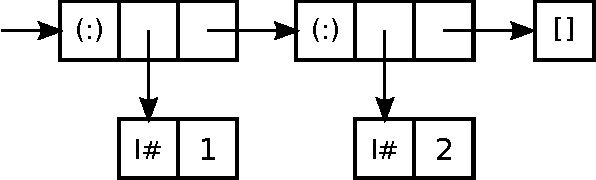
\includegraphics[scale=0.75]{diagrams/list12.pdf}
  \end{figure}

  \begin{itemize}
  \item Each box represents one machine word
  \item Arrows represent pointers
  \item Each constructor has one word overhead for e.g. GC information
  \end{itemize}
\end{frame}

\begin{frame}[fragile]
  \frametitle{Memory usage for data constructors}

  Rule of thumb: a constructor uses one word for a header, and one
  word for each field.  So e.g.
\begin{lstlisting}
data Uno = Uno a
data Due = Due a b
\end{lstlisting}

  an \lstinline!Uno! takes 2 words, and a \lstinline!Due! takes 3.

  \begin{itemize}
  \item Exception: a constructor with no fields (like
    \lstinline!Nothing! or \lstinline!True!) takes no space, as it's
    shared among all uses.
  \end{itemize}
\end{frame}

\begin{frame}[fragile]
  \frametitle{Unboxed types}

  GHC defines a number of \emph{unboxed} types.  These typically
  represent primitive machine types.

  \begin{itemize}
  \item By convention, the names of these types end with a
    \lstinline!#!.
  \item Most unboxed types take one word (except
    e.g. \lstinline!Double#! on 32-bit machines)
  \item Values of unboxed types are never lazy.
  \item The basic types are defined in terms unboxed types e.g.
  \begin{lstlisting}
data Int = I# Int#
  \end{lstlisting}
  \item We call types such as \lstinline!Int! \emph{boxed} types
  \end{itemize}
\end{frame}

\begin{frame}[fragile]
  \frametitle{Poll}

  How many machine words is needed to store a value of this data type:

\begin{lstlisting}
data IntPair = IP Int Int
\end{lstlisting}

  \begin{itemize}
  \item 3?
  \item 5?
  \item 7?
  \item 9?
  \end{itemize}
\end{frame}

\begin{frame}[fragile]
  \frametitle{IntPair memory layout}

  \begin{figure}
    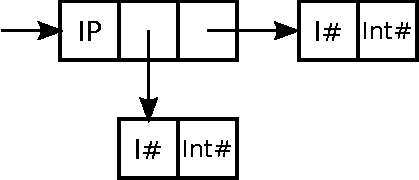
\includegraphics[scale=0.75]{diagrams/intpair.pdf}
  \end{figure}
  So an \lstinline!IntPair! value takes 7 words.
\end{frame}

\begin{frame}[fragile]
  \frametitle{Unpacking}

  GHC gives us some control over data representation via the
  \lstinline!UNPACK! pragma.

  \begin{itemize}
  \item The pragma unpacks the contents of a constructor into the
    field of another constructor, removing one level of indirection
    and one constructor header.
  \item Any strict, monomorphic, single-constructor field can be
    unpacked.
  \end{itemize}

  The pragma is added just before the bang pattern:

  \begin{lstlisting}
data Foo = Foo {-# UNPACK #-} !SomeType
  \end{lstlisting}
\end{frame}

\begin{frame}[fragile]
  \frametitle{Unpacking example}

  \begin{lstlisting}
data IntPair = IP Int Int
  \end{lstlisting}

  \begin{figure}
    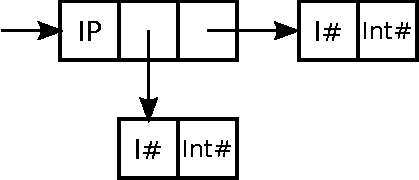
\includegraphics[scale=0.75]{diagrams/intpair.pdf}
  \end{figure}

  \begin{lstlisting}
data IntPair = IP {-# UNPACK #-} !Int
                  {-# UNPACK #-} !Int
  \end{lstlisting}

  \begin{figure}
    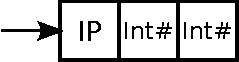
\includegraphics[scale=0.75]{diagrams/intpair-unpacked.pdf}
  \end{figure}
\end{frame}

\begin{frame}[fragile]
  \frametitle{Benefits of unpacking}

  When the pragma applies, it offers the following benefits:
  \begin{itemize}
  \item Reduced memory usage (4 words in the case of
    \lstinline!IntPair!)
  \item Fewer indirections
  \end{itemize}

  Caveat: There are cases where unpacking hurts performance e.g. if
  the fields are passed to a non-strict function.
\end{frame}


%%%%%%%%%%%%%%%%%%%%%%%%%%%%%%%%%%%%%%%%%%%%%%%%%%%%%%%%%%%%%%%%%%%%%%%%
% Benchmarking

\begin{frame}[fragile]
  \frametitle{Benchmarking}

  In principle, measuring code-execution time is trivial:
  \begin{enumerate}
  \item Record the start time.
  \item Execute the code.
  \item Record the stop time.
  \item Compute the time difference.
  \end{enumerate}
\end{frame}

\begin{frame}[fragile]
  \frametitle{A naive benchmark}

\begin{verbatim}
import time

def bench(f):
  start = time.time()
  f()
  end = time.time()
  print (end - start)
\end{verbatim}
\end{frame}

\begin{frame}
  \frametitle{Benchmarking gotchas}

  Potential problems with this approach:
  \begin{itemize}
  \item The clock resolution might be too low.
  \item The measurement overhead might skew the results.
  \item The compiler might detect that the result of the function
    isn't used and remove the call completely!
  \item Another process might get scheduled while the benchmark is
    running.
  \item GC costs might not be completely accounted for.
  \item Caches might be warm/cold.
  \end{itemize}
\end{frame}

\begin{frame}[fragile]
  \frametitle{Statistically robust benchmarking}

  The Criterion benchmarking library:
  \begin{itemize}
  \item Figures out how many times to run your function
  \item Adjusts for measurement overhead
  \item Computes confidence intervals
  \item Detects outliers
  \item Graphs the results
  \end{itemize}

\begin{verbatim}
cabal install -f-Chart Criterion
\end{verbatim}
\end{frame}

\begin{frame}[fragile]
  \frametitle{Benchmarking our favorite function}

  \begin{lstlisting}
import Criterion.Main

fib :: Int -> Int
fib 0 = 0
fib 1 = 1
fib n = fib (n-1) + fib (n-2)

main = defaultMain [
      bench "fib 10" (whnf fib 10)
    ]
  \end{lstlisting}
\end{frame}

\begin{frame}[fragile]
  \frametitle{Benchmark output, part 1}

  \begin{verbatim}
$ ./Fibber
warming up
estimating clock resolution...
mean is 8.638120 us (80001 iterations)
found 1375 outliers among 79999 samples (1.7%)
  1283 (1.6%) high severe
estimating cost of a clock call...
mean is 152.6399 ns (63 iterations)
found 3 outliers among 63 samples (4.8%)
  3 (4.8%) high mild
  \end{verbatim}
\end{frame}

\begin{frame}[fragile]
  \frametitle{Benchmark output, part 2}

  \begin{verbatim}
benchmarking fib 10
collecting 100 samples, 9475 iterations each, in
estimated 863.8696 ms
bootstrapping with 100000 resamples
mean: 925.4310 ns, lb 922.1965 ns, ub 930.9341 ns,
ci 0.950
std dev: 21.06324 ns, lb 14.54610 ns, ub 35.05525 ns,
ci 0.950
found 8 outliers among 100 samples (8.0%)
  7 (7.0%) high severe
variance introduced by outliers: 0.997%
variance is unaffected by outliers
  \end{verbatim}
\end{frame}

\begin{frame}[fragile]
  \frametitle{Evaluation depth}

  \begin{lstlisting}
bench "fib 10" (whnf fib 10)
  \end{lstlisting}

  \begin{itemize}
  \item \lstinline!whnf! evaluates the result to weak head normal form
    (i.e. to the outmost data constructor).
  \item If the benchmark generates a large data structure (e.g. a
    list), you can use \lstinline!nf! instead to force the generation
    of the whole data structure.
  \item It's important to think about what should get evaluated in the
    benchmark to ensure your benchmark reflects the use case you care
    about.
  \end{itemize}
\end{frame}

\begin{frame}[fragile]
  \frametitle{Benchmark: creating a list of 10k elements}

  \begin{lstlisting}
import Criterion.Main

main = defaultMain [
    bench "whnf" (whnf (replicate n) 'a')
  , bench "nf" (nf (replicate n) 'a')
  ]
  where n = 10000
  \end{lstlisting}

  The expression \lstinline!replicate n x! creates a list of n copies
  of x.
\end{frame}

\begin{frame}[fragile]
  \frametitle{The difference between whnf and nf}

  \begin{verbatim}
$ ./BuildList
benchmarking whnf
mean: 15.04583 ns, lb 14.97536 ns, ub 15.28949 ns, ...
std dev: 598.2378 ps, lb 191.2617 ps, ub 1.357806 ns, ...

benchmarking nf
mean: 158.3137 us, lb 158.1352 us, ub 158.5245 us, ...
std dev: 993.9415 ns, lb 834.4037 ns, ub 1.242261 us, ...
  \end{verbatim}

  Since \lstinline!replicate! generates the list lazily, the first
  benchmark only creates a single element
\end{frame}

\begin{frame}[fragile]
  \frametitle{A note about the whnf function}

  The \lstinline!whnf! function is somewhat peculiar:
  \begin{itemize}
  \item It takes the function to benchmark, applied to its first n-1
    arguments, as its first argument
  \item It takes the last, \emph{n}th, argument as its second argument
  \end{itemize}
  For example:
  \begin{lstlisting}
bench "product" (whnf (foldl (*) 1) [1..10000])
  \end{lstlisting}
By separating the last arguments from the rest, Criterion tries to
prevent GHC from evaluating the function being benchmarked only once.
\end{frame}

\begin{frame}[fragile]
  \frametitle{Exercise: foldl vs foldl'}

  Benchmark the performance of \lstinline!foldl (+) 0 [1..10000]! and
  \lstinline!foldl' (+) 0 [1..10000]!.  Start with:

  \begin{lstlisting}
import Criterion.Main
import Prelude hiding (foldl)

foldl, foldl' :: (a -> b -> a) -> a -> [b] -> a
foldl f z = ...
foldl' f z = ...
                       
main = defaultMain [
    bench "foldl" ...
  , bench "foldl'" ...
  ]
  \end{lstlisting}

  Compiling and running:
  \begin{verbatim}
$ ghc -O --make Fold.hs && ./Fold
  \end{verbatim}
\end{frame}

\begin{frame}[fragile]
  \frametitle{Solution}

  \begin{lstlisting}
import Criterion.Main
import Prelude hiding (foldl)

foldl, foldl' :: (a -> b -> a) -> a -> [b] -> a

foldl f z []     = z
foldl f z (x:xs) = foldl f (f z x) xs

foldl' f z []     = z
foldl' f z (x:xs) = let z' = f z x
                    in seq z' (foldl' f z' xs)
                       
main = defaultMain [
    bench "foldl" (whnf (foldl (+) 0) [1..10000])
  , bench "foldl'" (whnf (foldl' (+) 0) [1..10000])
  ]
  \end{lstlisting}
\end{frame}

\begin{frame}[fragile]
  \frametitle{Solution timings}

  \begin{verbatim}
benchmarking foldl
mean: 493.6532 us, lb 488.0841 us, ub 500.2349 us, ...
std dev: 31.11368 us, lb 26.20585 us, ub 42.98257 us, ...

benchmarking foldl'
mean: 121.3693 us, lb 120.8598 us, ub 122.6117 us, ...
std dev: 3.816444 us, lb 1.889005 us, ub 7.650491 us, ...
  \end{verbatim}
\end{frame}

%%%%%%%%%%%%%%%%%%%%%%%%%%%%%%%%%%%%%%%%%%%%%%%%%%%%%%%%%%%%%%%%%%%%%%%%
% Core

\begin{frame}
  \frametitle{GHC Core}

  \begin{itemize}
  \item GHC uses an intermediate language, called ``Core,'' as its
    internal representation during several compilation stages
  \item Core resembles a subset of Haskell
  \item The compiler performs many of its optimizations by repeatedly
    rewriting the Core code
  \end{itemize}
\end{frame}

\begin{frame}
  \frametitle{Why knowing how to read Core is important}

  Reading the generated Core lets you answer many questions, for
  example:
  \begin{itemize}
  \item When are expressions evaluated
  \item Is this function argument accessed via an indirection
  \item Did my function get inlined
  \end{itemize}
\end{frame}

\begin{frame}[fragile]
  \frametitle{Convincing GHC to show us the Core}

  Given this ``program''

  \begin{lstlisting}
module Sum where

import Prelude hiding (sum)

sum :: [Int] -> Int
sum []     = 0
sum (x:xs) = x + sum xs
  \end{lstlisting}

  we can get GHC to output the Core by adding the
  \texttt{-ddump-simpl} flag
  \begin{verbatim}
$ ghc -O --make Sum.hs -ddump-simpl
  \end{verbatim}
\end{frame}

\begin{frame}[fragile]
  \frametitle{A first taste of Core, part 1}
  \begin{verbatim}
Sum.sum :: [GHC.Types.Int] -> GHC.Types.Int
GblId
[Arity 1
 Worker Sum.$wsum
 NoCafRefs
 Str: DmdType Sm]
Sum.sum =
  __inline_me (\ (w_sgJ :: [GHC.Types.Int]) ->
    case Sum.$wsum w_sgJ of ww_sgM { __DEFAULT ->
    GHC.Types.I# ww_sgM
    })
  \end{verbatim}
\end{frame}

\begin{frame}[fragile]
  \frametitle{A first taste of Core, part 2}
  \begin{verbatim}
Rec {
Sum.$wsum :: [GHC.Types.Int] -> GHC.Prim.Int#
GblId
[Arity 1
 NoCafRefs
 Str: DmdType S]
Sum.$wsum = \ (w_sgJ :: [GHC.Types.Int]) ->
    case w_sgJ of _ {
      [] -> 0;
      : x_ade xs_adf ->
        case x_ade of _ { GHC.Types.I# x1_agv ->
        case Sum.$wsum xs_adf of ww_sgM { __DEFAULT ->
        GHC.Prim.+# x1_agv ww_sgM
        }
        }
    }
end Rec }
  \end{verbatim}
\end{frame}

\begin{frame}[fragile]
  \frametitle{Reading Core: a guide}

  \begin{itemize}
  \item All names a fully qualified (e.g. \lstinline!GHC.Types.Int!
    instead of just \lstinline!Int!)
  \item The parts after the function type declaration and before the
    function definition are annotations e.g.
    \begin{lstlisting}
GblId
[Arity ...]
    \end{lstlisting}
    We'll ignore those for now
  \item Lots of the names are generated by GHC
    (e.g. \lstinline!w_sgJ!).
  \end{itemize}
  Note: The Core syntax changes slightly with new compiler releases.
\end{frame}

\begin{frame}
  \frametitle{Tips for reading Core}

  Three tips for reading Core:
  \begin{itemize}
  \item Open and edit it in your favorite editor to simplify it
    (e.g. rename variables to something sensible).
  \item Use the ghc-core package on Hackage
  \item Use the GHC Core major mode in Emacs (ships with haskell-mode)
  \end{itemize}
\end{frame}

\begin{frame}[fragile]
  \frametitle{Cleaned up Core for sum}

  \begin{verbatim}
$wsum :: [Int] -> Int#
$wsum = \ (xs :: [Int]) ->
  case xs of _
    [] -> 0
    : x xs' -> case x of _
      I# x# -> case $wsum xs' of n#
        __DEFAULT -> +# x# n#

sum :: [Int] -> Int
sum = __inline_me (\ (xs :: [Int]) ->
        case $wsum xs of n#
          __DEFAULT -> I# n#)
  \end{verbatim}
\end{frame}

\begin{frame}[fragile]
  \frametitle{Core for sum explained}

  \begin{itemize}
  \item Convention: A variable name that ends with \# stands for an
    unboxed value.
  \item GHC has split \lstinline!sum! into two parts: a wrapper,
    \texttt{sum}, and a worker, \texttt{\$wsum}.
  \item The worker returns an unboxed integer, which the wrapper wraps
    in an \lstinline!I#! constructor.
  \item \texttt{+\#} is addition for unboxed integers (i.e. a single
    assembler instruction).
  \item The worker is not tail recursive, as it performs an addition
    after calling itself recursively.
  \item GHC has added a note that \texttt{sum} should be inlined.
  \end{itemize}
\end{frame}

\begin{frame}[fragile]
  \frametitle{Core, case, and evaluation}

  In core, \texttt{case} always means ``evaluate''.  Read
\begin{verbatim}
case xs of _
  [] -> ...
  : x xs' -> ...
\end{verbatim}
  as: evaluate \texttt{xs} and then evaluate one of the branches.

  \begin{itemize}
  \item Case statements are the only place where evaluation takes
    place.
  \item \emph{Except} when working with unboxed types where e.g.
\begin{verbatim}
f :: Int# -> ...
f (x# +# n#)
\end{verbatim}
    should be read as: evaluate \texttt{x\# +\# n\#} and then apply
    the function \texttt{f} to the result.
  \end{itemize}
\end{frame}

\begin{frame}[fragile]
  \frametitle{Tail recursive sum}

  \begin{lstlisting}
module TRSum where

import Prelude hiding (sum)

sum :: [Int] -> Int
sum = sum' 0
  where
    sum' acc []     = acc
    sum' acc (x:xs) = sum' (acc + x) xs
  \end{lstlisting}

  Compiling:
  \begin{verbatim}
$ ghc -O --make TRSum.hs -ddump-simpl
  \end{verbatim}
\end{frame}

\begin{frame}[fragile]
  \frametitle{Core for tail recursive sum}

  \begin{verbatim}
sum1 :: Int; sum1 = I# 0

$wsum' :: Int# -> [Int] -> Int#
$wsum' = \ (acc# :: Int#) (xs :: [Int]) ->
  case xs of _
    [] -> acc#
    : x xs' -> case x of _
      I# x# -> $wsum' (+# acc# x#) xs'

sum_sum' :: Int -> [Int] -> Int
sum_sum' = __inline_me (\ (acc :: Int) (xs :: [Int]) ->
  case acc of _
    I# acc# -> case $wsum' acc# xs of n#
      __DEFAULT -> I# n#)
 
sum :: [Int] -> Int
sum = __inline_me (sum_sum' sum1)
  \end{verbatim}
\end{frame}

\begin{frame}[fragile]
  \frametitle{Core for tail recursive sum explained}

  \begin{itemize}
  \item \texttt{\$wsum}'s first argument is an unboxed integer, which
    will be passed in a register if one is available.
  \item The recursive call to \texttt{\$wsum} is now tail recursive.
  \end{itemize}
\end{frame}

\begin{frame}[fragile]
  \frametitle{Polymorphic functions}

  In Core, polymorphic functions get an extra argument for each type
  parameter e.g.

\begin{lstlisting}
id :: a -> a
id x = x
\end{lstlisting}

  becomes

\begin{verbatim}
id :: forall a. a -> a
id = \ (@ a) (x :: a) -> x
\end{verbatim}

  This parameter is used by the type system and can be ignored.
\end{frame}

\begin{frame}[fragile]
  \frametitle{Exercise}

  Compare the Core generated by foldl and foldl' and find where they
  differ.  Start with:

  \begin{lstlisting}
module FoldCore where

import Prelude hiding (foldl)

foldl, foldl' :: (a -> b -> a) -> a -> [b] -> a
foldl = ...
foldl' = ...
  \end{lstlisting}

  Compile with:
  \begin{verbatim}
$ ghc -O --make FoldCore.hs -ddump-simpl
  \end{verbatim}
\end{frame}

\begin{frame}[fragile]
  \frametitle{Solution}

  The difference is in the recursive call:
  \begin{itemize}
  \item \lstinline!foldl'!:
  \begin{verbatim}
: x xs ->
  case f z x of z'
     __DEFAULT -> foldl' f z'
  \end{verbatim}
  \item \lstinline!foldl!:
  \begin{verbatim}
: x xs -> foldl f (f z x) xs
  \end{verbatim}
  \end{itemize}
\end{frame}

%%%%%%%%%%%%%%%%%%%%%%%%%%%%%%%%%%%%%%%%%%%%%%%%%%%%%%%%%%%%%%%%%%%%%%%%
% Profiling

%%%%%%%%%%%%%%%%%%%%%%%%%%%%%%%%%%%%%%%%%%%%%%%%%%%%%%%%%%%%%%%%%%%%%%%%

\begin{frame}
  \frametitle{Profiling}

  \begin{itemize}
  \item Profiling lets us find performance hotspots.
  \item Typically used when you already have performance problems.
  \end{itemize}
\end{frame}

\begin{frame}[fragile]
  \frametitle{Using profiling to find a space leak}

  \begin{lstlisting}
import System.Environment

main = do
    [d] <- map read `fmap` getArgs
    print (mean [1..d])

mean :: [Double] -> Double
mean xs = sum xs / fromIntegral (length xs)
  \end{lstlisting}

  Compiling:
  \begin{verbatim}
$ ghc -O --make SpaceLeak.hs -rtsopts
  \end{verbatim}
\end{frame}

\begin{frame}[fragile]
  \frametitle{Simple garbage collector statistics}

  \begin{verbatim}
$ ./SpaceLeak 1e7 +RTS -sstderr
./SpaceLeak 1e7 +RTS -sstderr 
5000000.5
     763,231,552 bytes allocated in the heap
     656,658,372 bytes copied during GC
     210,697,724 bytes maximum residency (9 sample(s))
       3,811,244 bytes maximum slop
             412 MB total memory in use (3 MB lost due
                 to fragmentation)

  Generation 0:  1447 collections,     0 parallel,
                 0.43s,  0.44s elapsed
  Generation 1:     9 collections,     0 parallel,
                 0.77s,  1.12s elapsed
  \end{verbatim}
\end{frame}

\begin{frame}[fragile]
  \frametitle{Simple garbage collector statistics cont.}

  \begin{verbatim}
  INIT  time    0.00s  (  0.00s elapsed)
  MUT   time    0.54s  (  0.54s elapsed)
  GC    time    1.20s  (  1.56s elapsed)
  EXIT  time    0.00s  (  0.00s elapsed)
  Total time    1.74s  (  2.10s elapsed)

  %GC time      69.0%  (74.1% elapsed)

  Alloc rate    1,417,605,200 bytes per MUT second

  Productivity  30.9% of total user, 25.6% of total
                elapsed
  \end{verbatim}
\end{frame}

\begin{frame}
  \frametitle{The important bits}

  \begin{itemize}
  \item The program used a maximum of 412 MB of heap
  \item The were 1447 minor collections
  \item The were 9 major collections
  \item 69\% of the time was spent doing garbage collection!
  \end{itemize}
\end{frame}

\begin{frame}[fragile]
  \frametitle{Time profiling}

  \begin{verbatim}
$ ghc -O --make SpaceLeak.hs -prof -auto-all -caf-all \
  -fforce-recomp
$ ./SpaceLeak 1e7 +RTS -p
Stack space overflow: current size 8388608 bytes.
Use `+RTS -Ksize -RTS' to increase it.
  \end{verbatim}

  Lets increase the stack size to make the program finish
  \begin{verbatim}
$ ./SpaceLeak 1e7 +RTS -p -K400M
  \end{verbatim}
\end{frame}

\begin{frame}[fragile]
  \frametitle{Time profiling results}

  \begin{verbatim}
COST CENTRE   MODULE     %time %alloc

CAF:main_sum  Main        81.0   29.6
mean          Main        14.3    0.0
CAF           GHC.Double   4.8   70.4
  \end{verbatim}

  The information isn't conclusive, but it seems like the runtime is
  due to the \lstinline!sum! function and the allocation of lots of
  \lstinline!Double!s.
\end{frame}

\begin{frame}[fragile]
  \frametitle{Space profiling}

  Lets take another perspective by profiling the program space usage:
  \begin{verbatim}
$ ./SpaceLeak 1e7 +RTS -p -K400M -hy
  \end{verbatim}

  Generate a pretty graph of the result:
  \begin{verbatim}
$ hp2ps -c SpaceLeak.hp
  \end{verbatim}
\end{frame}

\begin{frame}
  \frametitle{Space usage graph}

  \begin{figure}
    \includegraphics[scale=1.0]{diagrams/SpaceLeak.eps}
  \end{figure}
\end{frame}

\begin{frame}[fragile]
  \frametitle{Space leak explained}

  From the graph we can confirm that a list of \lstinline!Double!s are
  being allocated but not freed immediately.  The culprit is our
  formulation of \lstinline!mean!

  \begin{lstlisting}
mean :: [Double] -> Double
mean xs = sum xs / fromIntegral (length xs)
  \end{lstlisting}

  \lstinline!sum! causes the list \lstinline!xs! to be generated, but
  the list elements cannot be freed immediately as it's needed later
  by \lstinline!length!.
\end{frame}

\begin{frame}[fragile]
  \frametitle{Space leak fix}

  We've already seen the solution: compute the sum and the length at
  the same time:
  \begin{lstlisting}
mean :: [Double] -> Double
mean xs = s / fromIntegral l
  where
    (s, l) = foldl' step (0, 0) xs
    step (!s, !l) a = (s+a, l+1)
  \end{lstlisting}
\end{frame}

\begin{frame}
  \frametitle{Writing high-performance code}

  \begin{enumerate}
  \item Profile to find performance hotspots
  \item Write a benchmark for the offending function
  \item Improve the performance, by adjusting evaluation order and
    unboxing
  \item Look at the generated Core
  \item Run benchmarks to confirm speedup
  \item Repeat
  \end{enumerate}
\end{frame}

\begin{frame}
  \frametitle{References / more content}

  \begin{itemize}
  \item The Haskell Wiki:
    http://www.haskell.org/haskellwiki/Performance
  \item Real World Haskell, chapter 25
  \item My blog:
    http://blog.johantibell.com/
  \end{itemize}
\end{frame}

\begin{frame}
  \frametitle{Bonus: Argument unboxing}

  \begin{itemize}
  \item Strict function arguments are great for performance.
  \item GHC can often represents these as unboxed values, passed
    around in registers.
  \item GHC can often infer which arguments are stricts, but can
    sometimes need a little help.
  \end{itemize}
\end{frame}

\begin{frame}[fragile]
  \frametitle{Making functions stricter}

  As we saw earlier, \lstinline!insert! is not strict in its first
  argument.
  \begin{lstlisting}
data BST = Leaf | Node Int BST BST

insert :: Int -> BST -> BST
insert x Leaf   = Node x Leaf Leaf
insert x (Node x' l r)
    | x < x'    = Node x' (insert x l) r
    | x > x'    = Node x' l (insert x r)
    | otherwise = Node x l r
  \end{lstlisting}
  The first argument is represented as a boxed \lstinline!Int! value.
\end{frame}

\begin{frame}[fragile]
  \frametitle{Core for insert}

  \begin{verbatim}
insert :: Int -> BST -> BST
insert = \ (x :: Int) (t :: BST) ->
  case t of _
    Leaf -> Node x Leaf Leaf
    Node x' l r ->
      case x of _
        I# x# -> case x' of _
          I# x'# -> case <# x# x'# of _
            False -> case ># x# x'# of _
              False -> Node x l r
              True -> Node x' l (insert x r)
            True -> Node x' (insert x l) r
  \end{verbatim}
\end{frame}

\begin{frame}[fragile]
  \frametitle{Making functions stricter, part 2}

  We can make \lstinline!insert! strict in the firsst argument by
  using a bang pattern.
  \begin{lstlisting}
{-# LANGUAGE BangPatterns #-}

insert :: a -> BST a -> BST a
insert !x Leaf  = Node x Leaf Leaf
insert x (Node x' l r)
    | x < x'    = Node x' (insert x l) r
    | x > x'    = Node x' l (insert x r)
    | otherwise = Node x l r
  \end{lstlisting}
  Now both equations always cause \lstinline!x! to be evaluated.
\end{frame}

\begin{frame}[fragile]
  \frametitle{Core for stricter insert}

  \begin{verbatim}
$winsert :: Int# -> BST -> BST
$winsert = \ (x# :: Int#) (t :: BST) ->
  case t of _
    Leaf -> Node (I# x#) Leaf Leaf
    Node x' l r -> case x' of _
      I# x'# -> case <# x# x'# of _
        False -> case ># x# x'# of _
          False -> Node (I# x#) l r
          True -> Node x' l ($winsert x# r)
        True -> Node x' ($winsert x# l) r
  \end{verbatim}
\end{frame}

\begin{frame}[fragile]
  \frametitle{Benefits of strict functions}

  There are two main benefits of to making functions strict:
  \begin{itemize}
  \item No indirections when accessing arguments
  \item Less allocation
  \end{itemize}
\end{frame}

\end{document}

%%% Local Variables:
%%% mode: latex
%%% TeX-master: t
%%% TeX-PDF-mode: t
%%% End:
